\documentclass{standalone}
\usepackage{tikz}
\usetikzlibrary{patterns, positioning}


\begin{document}
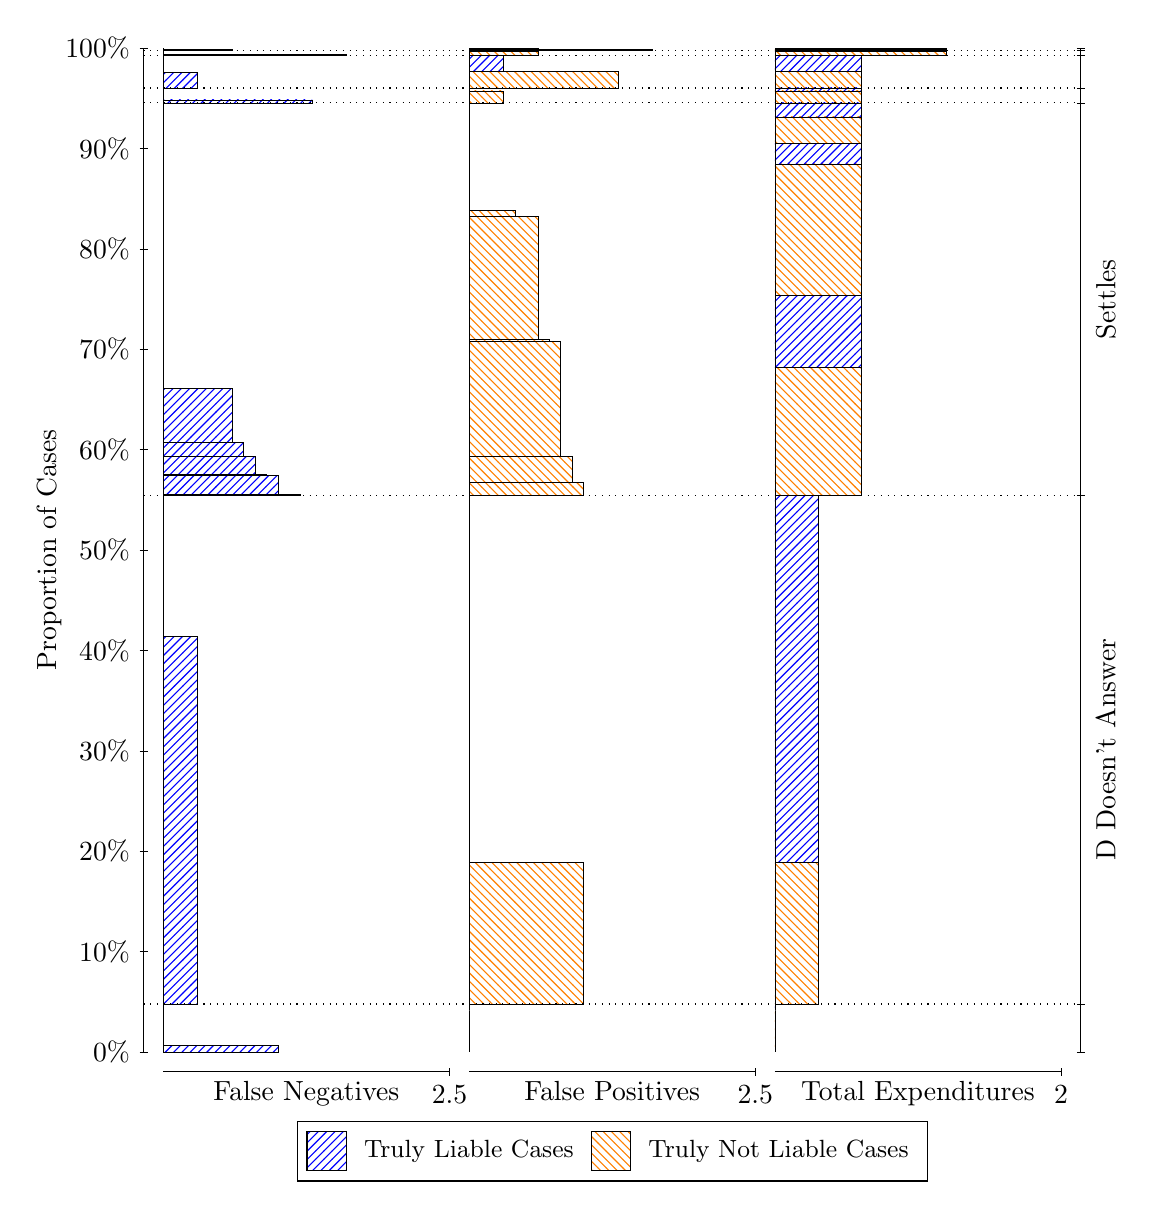
\begin{tikzpicture}
\draw[black, very thin] (1.5,1.75) -- (1.5,14.5);
\node[rotate=90, text=black, anchor=center] at (0.3, 8.125) {Proportion of Cases};
\draw[black, very thin] (1.45,1.75) -- (1.55,1.75);
\node[text=black, anchor=east] at (1.45, 1.75) {0\%};
\draw[black, very thin] (1.45,3.025) -- (1.55,3.025);
\node[text=black, anchor=east] at (1.45, 3.025) {10\%};
\draw[black, very thin] (1.45,4.3) -- (1.55,4.3);
\node[text=black, anchor=east] at (1.45, 4.3) {20\%};
\draw[black, very thin] (1.45,5.575) -- (1.55,5.575);
\node[text=black, anchor=east] at (1.45, 5.575) {30\%};
\draw[black, very thin] (1.45,6.85) -- (1.55,6.85);
\node[text=black, anchor=east] at (1.45, 6.85) {40\%};
\draw[black, very thin] (1.45,8.125) -- (1.55,8.125);
\node[text=black, anchor=east] at (1.45, 8.125) {50\%};
\draw[black, very thin] (1.45,9.4) -- (1.55,9.4);
\node[text=black, anchor=east] at (1.45, 9.4) {60\%};
\draw[black, very thin] (1.45,10.675) -- (1.55,10.675);
\node[text=black, anchor=east] at (1.45, 10.675) {70\%};
\draw[black, very thin] (1.45,11.95) -- (1.55,11.95);
\node[text=black, anchor=east] at (1.45, 11.95) {80\%};
\draw[black, very thin] (1.45,13.225) -- (1.55,13.225);
\node[text=black, anchor=east] at (1.45, 13.225) {90\%};
\draw[black, very thin] (1.45,14.5) -- (1.55,14.5);
\node[text=black, anchor=east] at (1.45, 14.5) {100\%};

\draw[black, very thin] (13.4,1.75) -- (13.4,14.5);
\draw[black, very thin] (13.35,1.75) -- (13.45,1.75);
\node[anchor=west] at (13.35, 1.75) {};
\draw[black, very thin] (13.35,2.3599) -- (13.45,2.3599);
\node[anchor=west] at (13.35, 2.3599) {};
\draw[black, very thin] (13.35,8.8188) -- (13.45,8.8188);
\node[anchor=west] at (13.35, 8.8188) {};
\draw[black, very thin] (13.35,13.803) -- (13.45,13.803);
\node[anchor=west] at (13.35, 13.803) {};
\draw[black, very thin] (13.35,13.993) -- (13.45,13.993);
\node[anchor=west] at (13.35, 13.993) {};
\draw[black, very thin] (13.35,14.402) -- (13.45,14.402);
\node[anchor=west] at (13.35, 14.402) {};
\draw[black, very thin] (13.35,14.468) -- (13.45,14.468);
\node[anchor=west] at (13.35, 14.468) {};
\draw[black, very thin] (13.35,14.5) -- (13.45,14.5);
\node[anchor=west] at (13.35, 14.5) {};

\draw[black, very thin, pattern color=blue, pattern=north east lines] (1.75,1.75) rectangle (3.2033,1.8312);
\draw[black, very thin, pattern color=orange, pattern=north west lines] (1.75,1.8312) rectangle (1.75,2.3599);
\draw[black, very thin, pattern color=blue, pattern=north east lines] (1.75,2.3599) rectangle (2.186,7.0232);
\draw[black, very thin, pattern color=orange, pattern=north west lines] (1.75,7.0232) rectangle (1.75,8.8188);
\draw[black, very thin, pattern color=blue, pattern=north east lines] (1.75,8.8188) rectangle (3.494,8.8314);
\draw[black, very thin, pattern color=blue, pattern=north east lines] (1.75,8.8314) rectangle (3.2033,9.0741);
\draw[black, very thin, pattern color=blue, pattern=north east lines] (1.75,9.0741) rectangle (3.058,9.0826);
\draw[black, very thin, pattern color=blue, pattern=north east lines] (1.75,9.0826) rectangle (2.9127,9.3134);
\draw[black, very thin, pattern color=blue, pattern=north east lines] (1.75,9.3134) rectangle (2.7673,9.4923);
\draw[black, very thin, pattern color=blue, pattern=north east lines] (1.75,9.4923) rectangle (2.622,10.181);
\draw[black, very thin, pattern color=orange, pattern=north west lines] (1.75,10.181) rectangle (1.75,13.803);
\draw[black, very thin, pattern color=blue, pattern=north east lines] (1.75,13.803) rectangle (3.6393,13.842);
\draw[black, very thin, pattern color=orange, pattern=north west lines] (1.75,13.842) rectangle (1.75,13.993);
\draw[black, very thin, pattern color=blue, pattern=north east lines] (1.75,13.993) rectangle (2.186,14.191);
\draw[black, very thin, pattern color=orange, pattern=north west lines] (1.75,14.191) rectangle (1.75,14.402);
\draw[black, very thin, pattern color=blue, pattern=north east lines] (1.75,14.402) rectangle (4.0753,14.417);
\draw[black, very thin, pattern color=orange, pattern=north west lines] (1.75,14.417) rectangle (1.75,14.468);
\draw[black, very thin, pattern color=blue, pattern=north east lines] (1.75,14.468) rectangle (2.622,14.485);
\draw[black, very thin, pattern color=orange, pattern=north west lines] (1.75,14.485) rectangle (1.75,14.5);
\draw[black, very thin, pattern color=orange, pattern=north west lines] (5.6333,1.75) rectangle (5.6333,2.2787);
\draw[black, very thin, pattern color=blue, pattern=north east lines] (5.6333,2.2787) rectangle (5.6333,2.3599);
\draw[black, very thin, pattern color=orange, pattern=north west lines] (5.6333,2.3599) rectangle (7.0867,4.1555);
\draw[black, very thin, pattern color=blue, pattern=north east lines] (5.6333,4.1555) rectangle (5.6333,8.8188);
\draw[black, very thin, pattern color=orange, pattern=north west lines] (5.6333,8.8188) rectangle (7.0867,8.9813);
\draw[black, very thin, pattern color=orange, pattern=north west lines] (5.6333,8.9813) rectangle (6.9413,9.3127);
\draw[black, very thin, pattern color=orange, pattern=north west lines] (5.6333,9.3127) rectangle (6.796,10.773);
\draw[black, very thin, pattern color=orange, pattern=north west lines] (5.6333,10.773) rectangle (6.6507,10.804);
\draw[black, very thin, pattern color=orange, pattern=north west lines] (5.6333,10.804) rectangle (6.5053,12.363);
\draw[black, very thin, pattern color=orange, pattern=north west lines] (5.6333,12.363) rectangle (6.2147,12.441);
\draw[black, very thin, pattern color=blue, pattern=north east lines] (5.6333,12.441) rectangle (5.6333,13.803);
\draw[black, very thin, pattern color=orange, pattern=north west lines] (5.6333,13.803) rectangle (6.0693,13.955);
\draw[black, very thin, pattern color=blue, pattern=north east lines] (5.6333,13.955) rectangle (5.6333,13.993);
\draw[black, very thin, pattern color=orange, pattern=north west lines] (5.6333,13.993) rectangle (7.5227,14.204);
\draw[black, very thin, pattern color=blue, pattern=north east lines] (5.6333,14.204) rectangle (6.0693,14.402);
\draw[black, very thin, pattern color=orange, pattern=north west lines] (5.6333,14.402) rectangle (6.5053,14.453);
\draw[black, very thin, pattern color=blue, pattern=north east lines] (5.6333,14.453) rectangle (5.6333,14.468);
\draw[black, very thin, pattern color=orange, pattern=north west lines] (5.6333,14.468) rectangle (7.9587,14.483);
\draw[black, very thin, pattern color=blue, pattern=north east lines] (5.6333,14.483) rectangle (6.5053,14.5);
\draw[black, very thin, pattern color=orange, pattern=north west lines] (9.5167,1.75) rectangle (9.5167,2.2787);
\draw[black, very thin, pattern color=blue, pattern=north east lines] (9.5167,2.2787) rectangle (9.5167,2.3599);
\draw[black, very thin, pattern color=orange, pattern=north west lines] (9.5167,2.3599) rectangle (10.062,4.1555);
\draw[black, very thin, pattern color=blue, pattern=north east lines] (9.5167,4.1555) rectangle (10.062,8.8188);
\draw[black, very thin, pattern color=orange, pattern=north west lines] (9.5167,8.8188) rectangle (10.607,10.442);
\draw[black, very thin, pattern color=blue, pattern=north east lines] (9.5167,10.442) rectangle (10.607,11.362);
\draw[black, very thin, pattern color=orange, pattern=north west lines] (9.5167,11.362) rectangle (10.607,13.03);
\draw[black, very thin, pattern color=blue, pattern=north east lines] (9.5167,13.03) rectangle (10.607,13.293);
\draw[black, very thin, pattern color=orange, pattern=north west lines] (9.5167,13.293) rectangle (10.607,13.625);
\draw[black, very thin, pattern color=blue, pattern=north east lines] (9.5167,13.625) rectangle (10.607,13.803);
\draw[black, very thin, pattern color=orange, pattern=north west lines] (9.5167,13.803) rectangle (10.607,13.955);
\draw[black, very thin, pattern color=blue, pattern=north east lines] (9.5167,13.955) rectangle (10.607,13.993);
\draw[black, very thin, pattern color=orange, pattern=north west lines] (9.5167,13.993) rectangle (10.607,14.204);
\draw[black, very thin, pattern color=blue, pattern=north east lines] (9.5167,14.204) rectangle (10.607,14.402);
\draw[black, very thin, pattern color=orange, pattern=north west lines] (9.5167,14.402) rectangle (11.697,14.453);
\draw[black, very thin, pattern color=blue, pattern=north east lines] (9.5167,14.453) rectangle (11.697,14.468);
\draw[black, very thin, pattern color=orange, pattern=north west lines] (9.5167,14.468) rectangle (11.697,14.483);
\draw[black, very thin, pattern color=blue, pattern=north east lines] (9.5167,14.483) rectangle (11.697,14.5);
\draw[black, dotted] (1.5,2.3599) -- (13.4,2.3599);
\draw[black, dotted] (1.5,8.8188) -- (13.4,8.8188);
\draw[black, dotted] (1.5,13.803) -- (13.4,13.803);
\draw[black, dotted] (1.5,13.993) -- (13.4,13.993);
\draw[black, dotted] (1.5,14.402) -- (13.4,14.402);
\draw[black, dotted] (1.5,14.468) -- (13.4,14.468);
\draw[black, very thin] (1.75,1.5) -- (5.3833,1.5);
\node[text=black, anchor=north] at (3.5667, 1.5) {False Negatives};
\draw[black, very thin] (5.3833,1.45) -- (5.3833,1.55);
\node[text=black, anchor=north] at (5.3833, 1.45) {2.5};

\draw[black, very thin] (5.6333,1.5) -- (9.2667,1.5);
\node[text=black, anchor=north] at (7.45, 1.5) {False Positives};
\draw[black, very thin] (9.2667,1.45) -- (9.2667,1.55);
\node[text=black, anchor=north] at (9.2667, 1.45) {2.5};

\draw[black, very thin] (9.5167,1.5) -- (13.15,1.5);
\node[text=black, anchor=north] at (11.333, 1.5) {Total Expenditures};
\draw[black, very thin] (13.15,1.45) -- (13.15,1.55);
\node[text=black, anchor=north] at (13.15, 1.45) {2};


\node[text=black, centered, rotate=90] at (13.72, 5.5894) {D Doesn't Answer};
\node[text=black, centered, rotate=90] at (13.72, 11.311) {Settles};





\draw (7.449999999999999,1.5) node[draw=none] (baseCoordinate) {};
\begin{scope}[align=center]
        \matrix[scale=0.5, draw=black, below=0.5cm of baseCoordinate, nodes={draw}, column sep=0.1cm]{
            \node[rectangle, draw, minimum width=0.5cm, minimum height=0.5cm, pattern color=blue, pattern=north east lines] {}; &
            \node[draw=none, font=\small, text=black] (B) {Truly Liable Cases}; &
            \node[rectangle, draw, minimum width=0.5cm, minimum height=0.5cm, pattern color=orange, pattern=north west lines] {}; &
            \node[draw=none, font=\small, text=black] (B) {Truly Not Liable Cases}; \\
            };
\end{scope}

\end{tikzpicture}
\end{document}